\section{AC/DC Power Circuit Application With LM2596\_5P0\_TRANS}
Hình 10.1 mô tả mạch cấp nguồn chuyển mạch LM2596 - 5.0 của Texas Instrument chưa hoàn chỉnh. Nó thiếu bộ điều chỉnh điện áp diode Zener và cuộn cảm giảm điện áp
biến thể. Đầu tiên, hãy thực hiện mô phỏng miền thời gian (tạm thời) với phần này chưa hoàn chỉnh.
mạch và tìm ra vấn đề với điện áp đầu ra (điểm đánh dấu điện áp ở R1).

\begin{figure}[h]
    \centering
    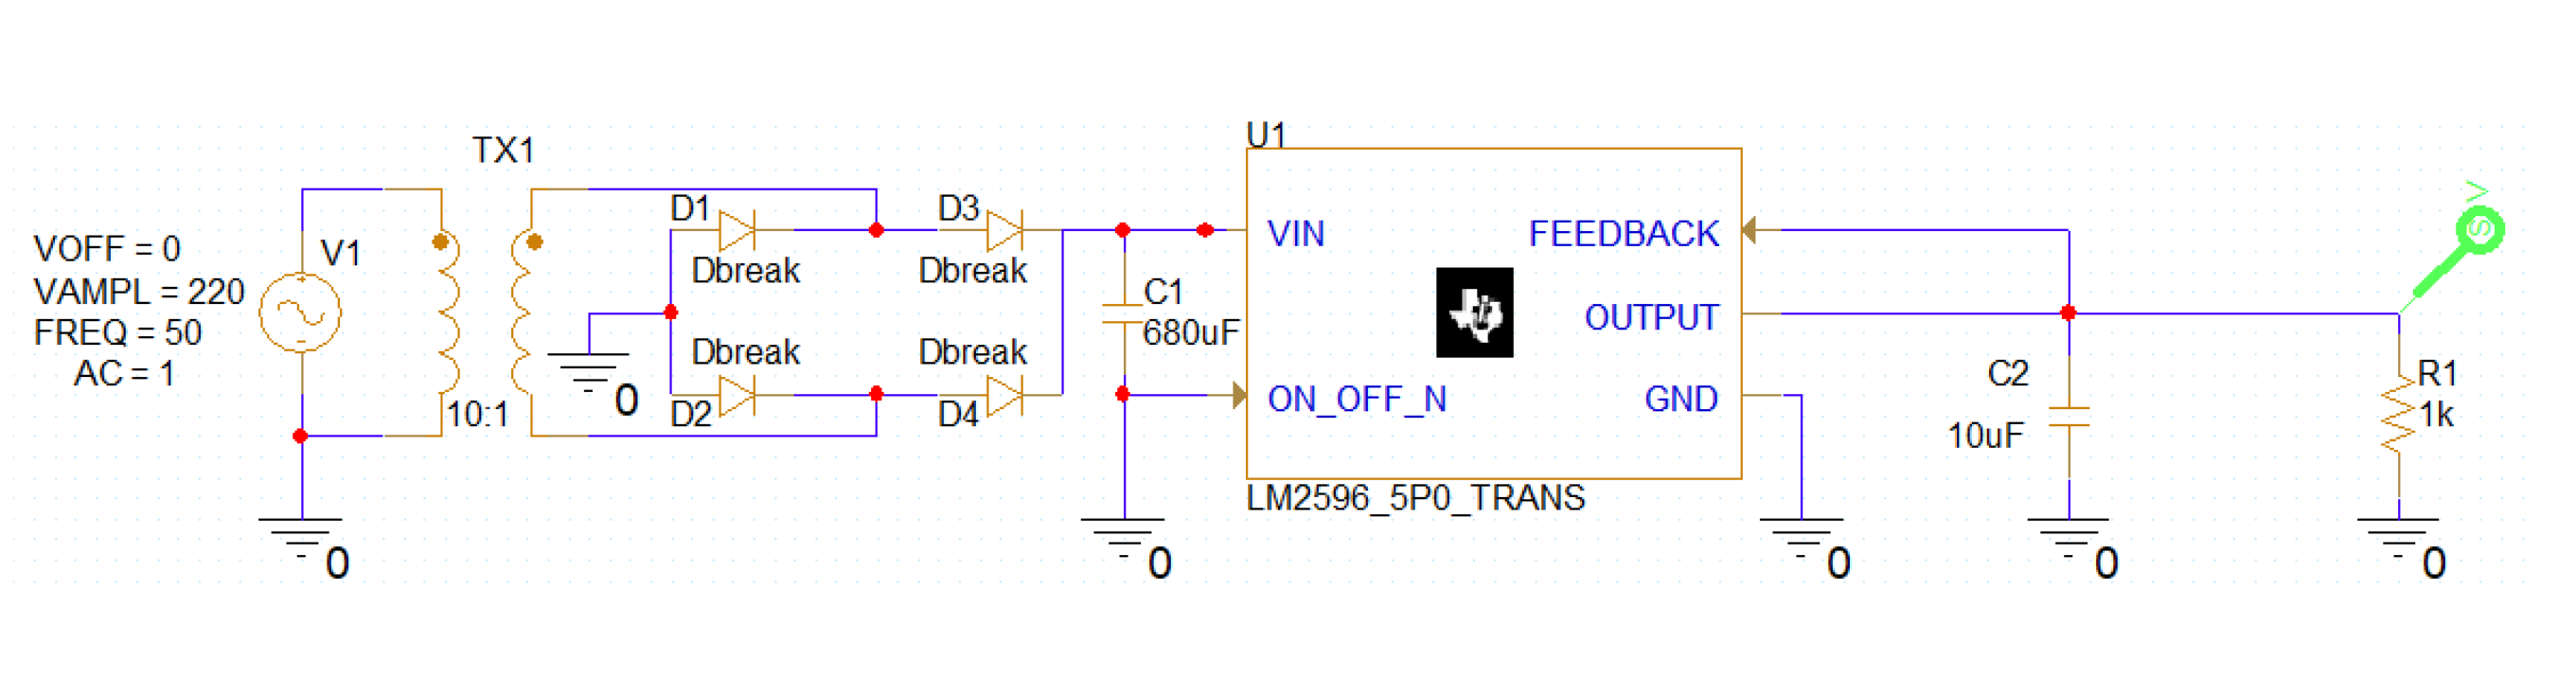
\includegraphics[scale=0.22]{graphics/ex10/f1.png}
    \caption{Mạch cấp nguồn chuyển mạch không hoàn chỉnh}
\end{figure}

\textbf{Tip:}

Để đặt bộ nguồn chuyển mạch IC LM2596 - 5.0, hãy vào \textbf{Place > PSpice Component...
> Search...} sau đó tìm kiếm LM2596\_5P0\_TRANS.

Nhưng trước khi bạn có thể thực hiện mô phỏng và phân tích nhất thời với mạch này, chúng ta sẽ
cần chú ý một số cài đặt nhỏ trên profile mô phỏng.

\begin{figure}[h]
    \centering
    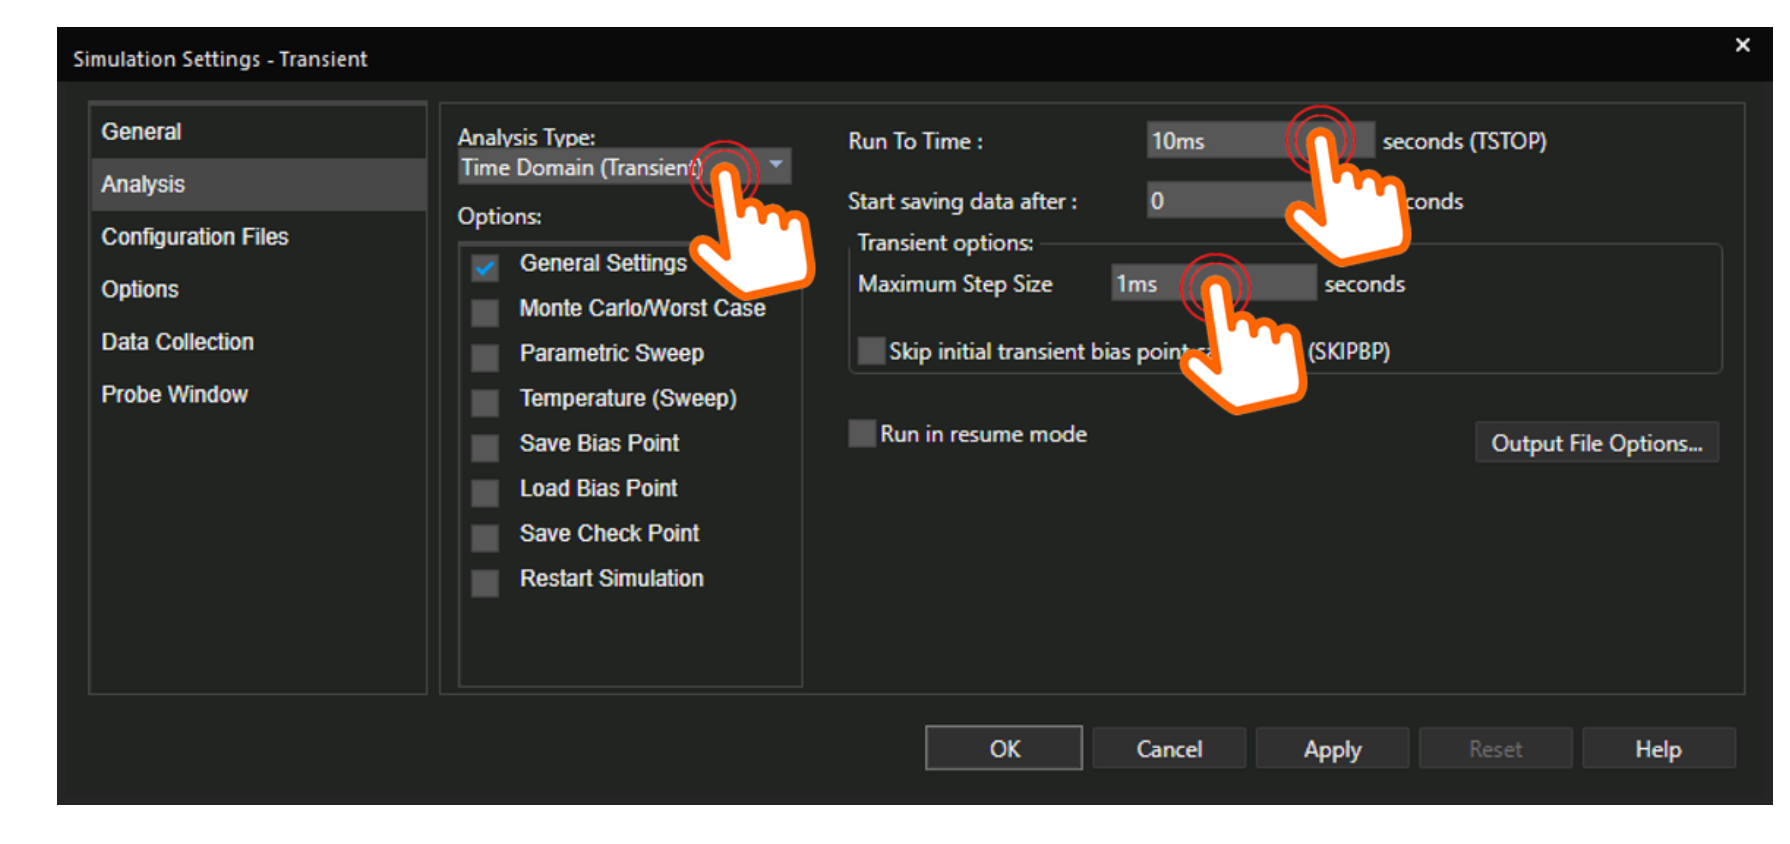
\includegraphics[scale=0.3]{graphics/ex10/f2.png}
    \caption{Đặt thời lượng mô phỏng nhất thời}
\end{figure}

\begin{figure}[ht]
    \centering
    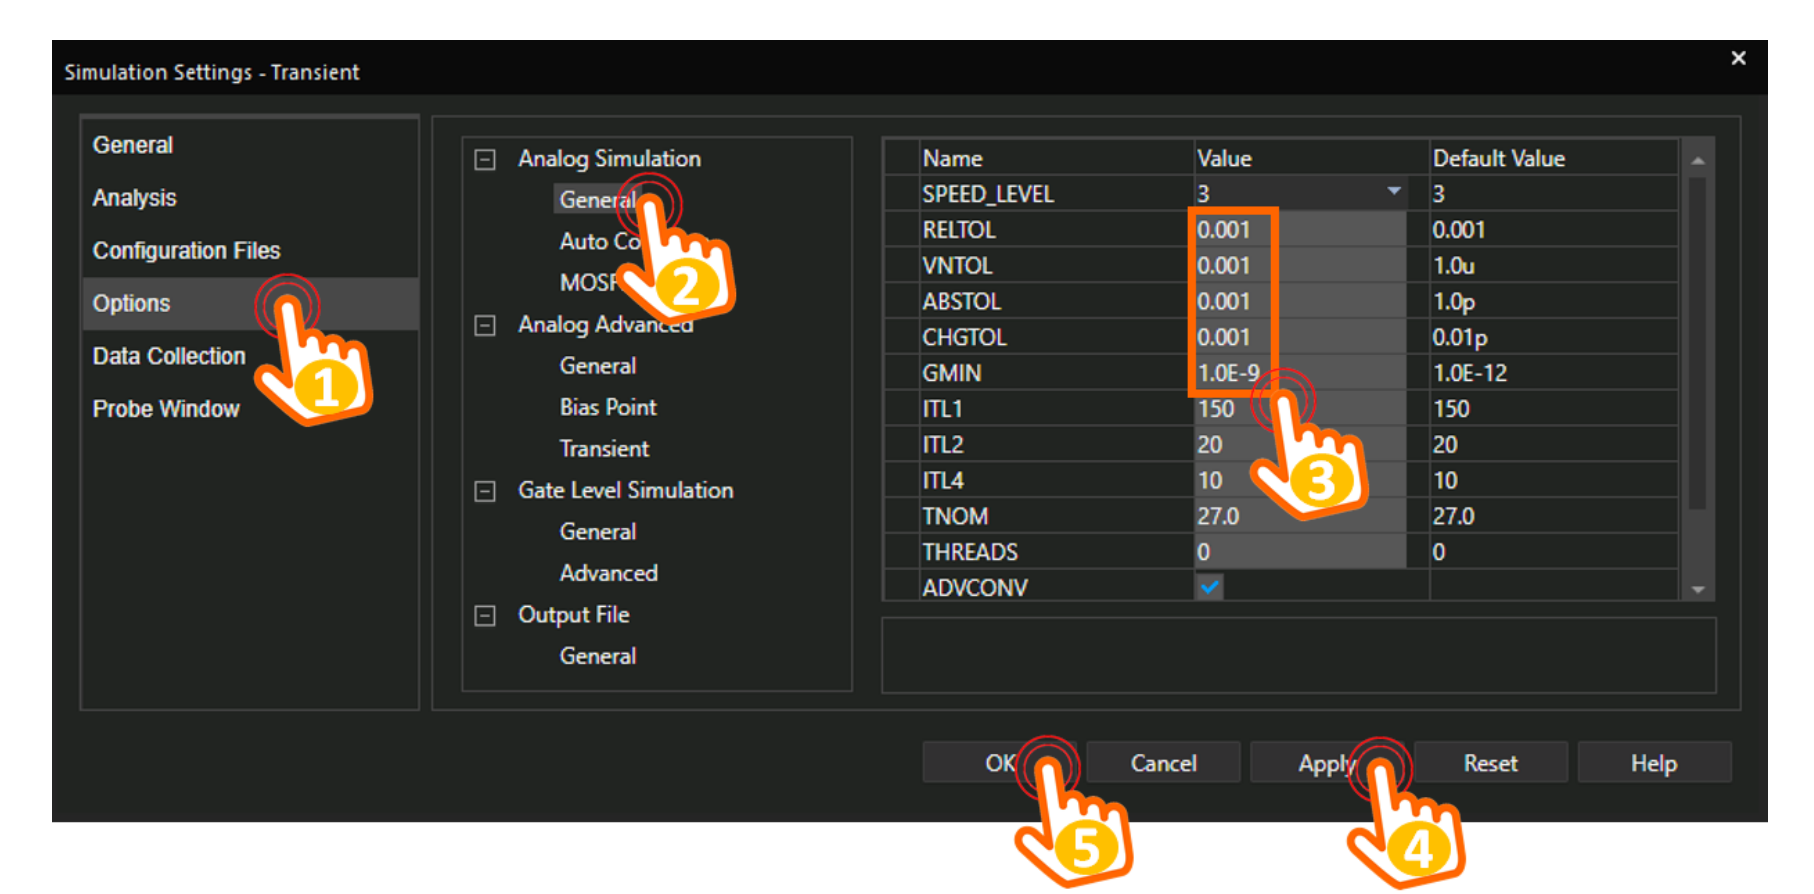
\includegraphics[scale=0.3]{graphics/ex10/f3.png}
    \caption{Đặt độ chính xác tính toán nhất thời}
\end{figure}
\pagebreak
\textbf{Kết quả mô phỏng: }

\begin{figure}[ht]
    \centering
    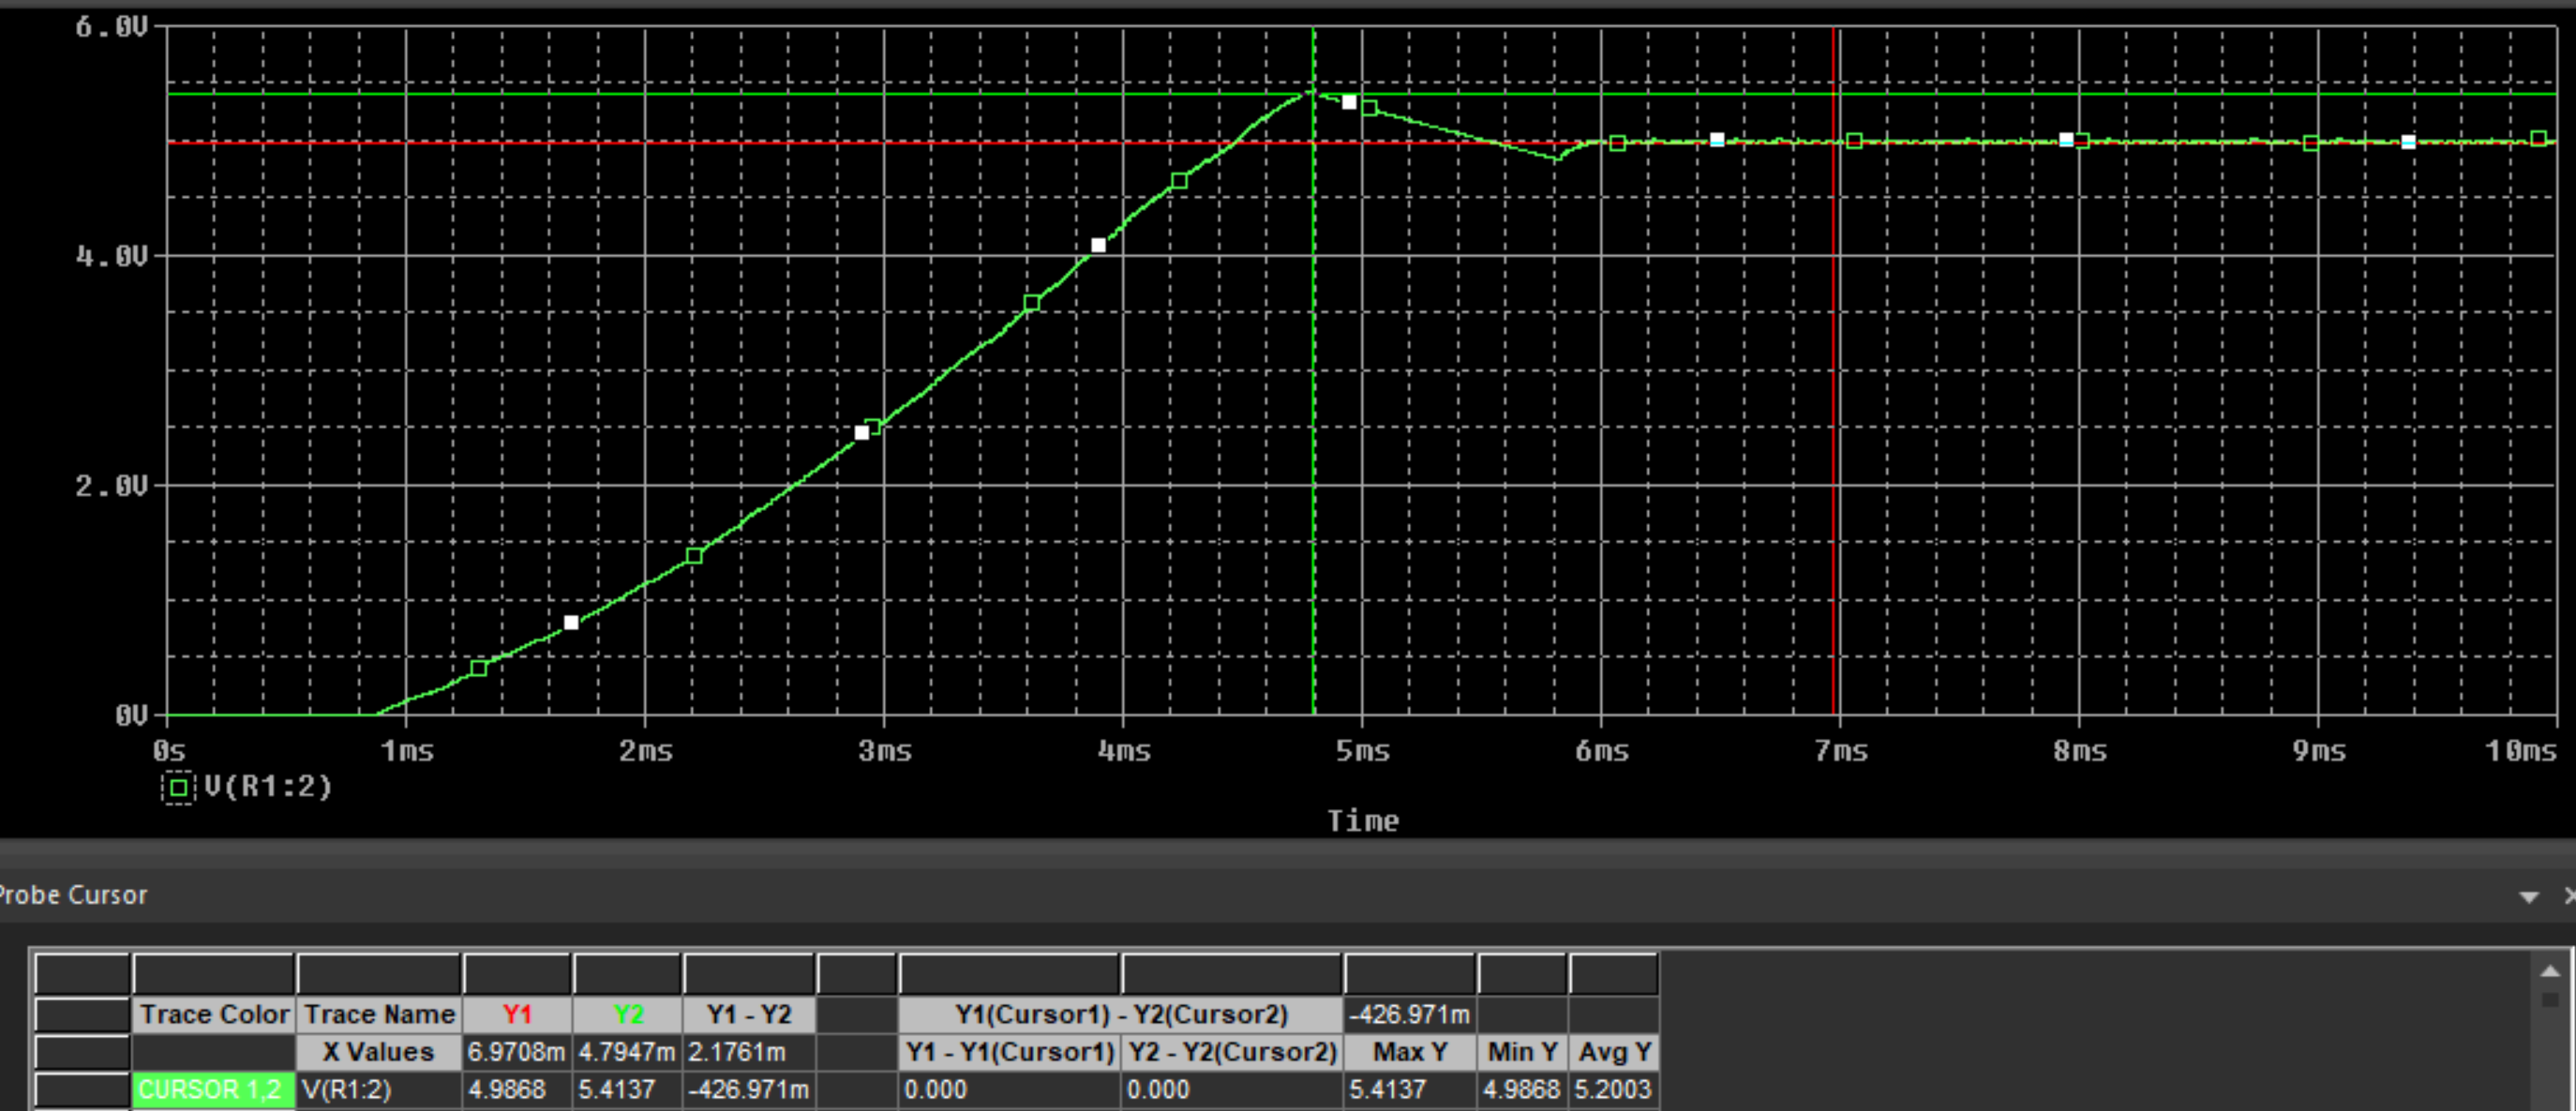
\includegraphics[scale=0.22]{graphics/ex10/f6.png}
    \caption{Kết quả mô phỏng của mạch trên}
\end{figure}

\textbf{Nhận xét và giải thích:} Đồ thị điện áp qua điện trở tăng nhanh trong khoảng 4ms đầu, sau đó giảm một chút rồi ổn định ở mức 5 (V) nhưng vẫn còn thay đổi một chút với sai số khoảng 0,03 (V).
\pagebreak

Tiếp theo, thêm một cuộn cảm 33µH vào mạch như trong Hình 10.5, sau đó chạy lại mô phỏng và giải thích mọi cải tiến.

\begin{figure}[ht]
    \centering
    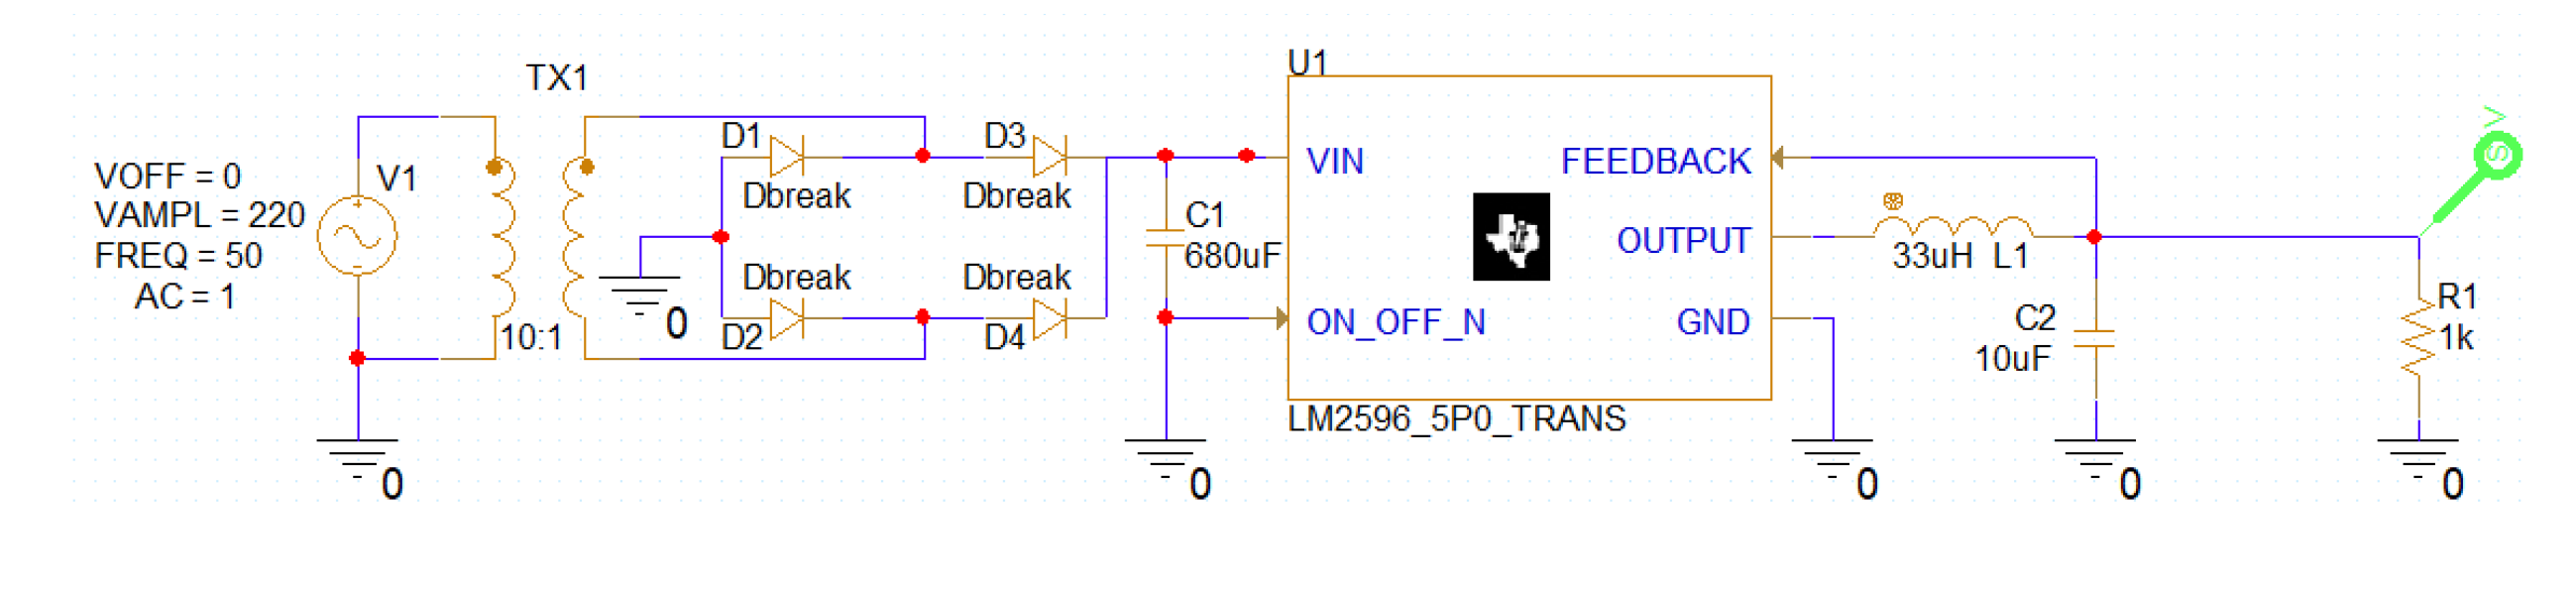
\includegraphics[scale=0.23]{graphics/ex10/f4.png}
    \caption{Một cuộn cảm 33µH được thêm vào mạch}
\end{figure}

\textbf{Kết quả mô phỏng: }

\begin{figure}[ht]
    \centering
    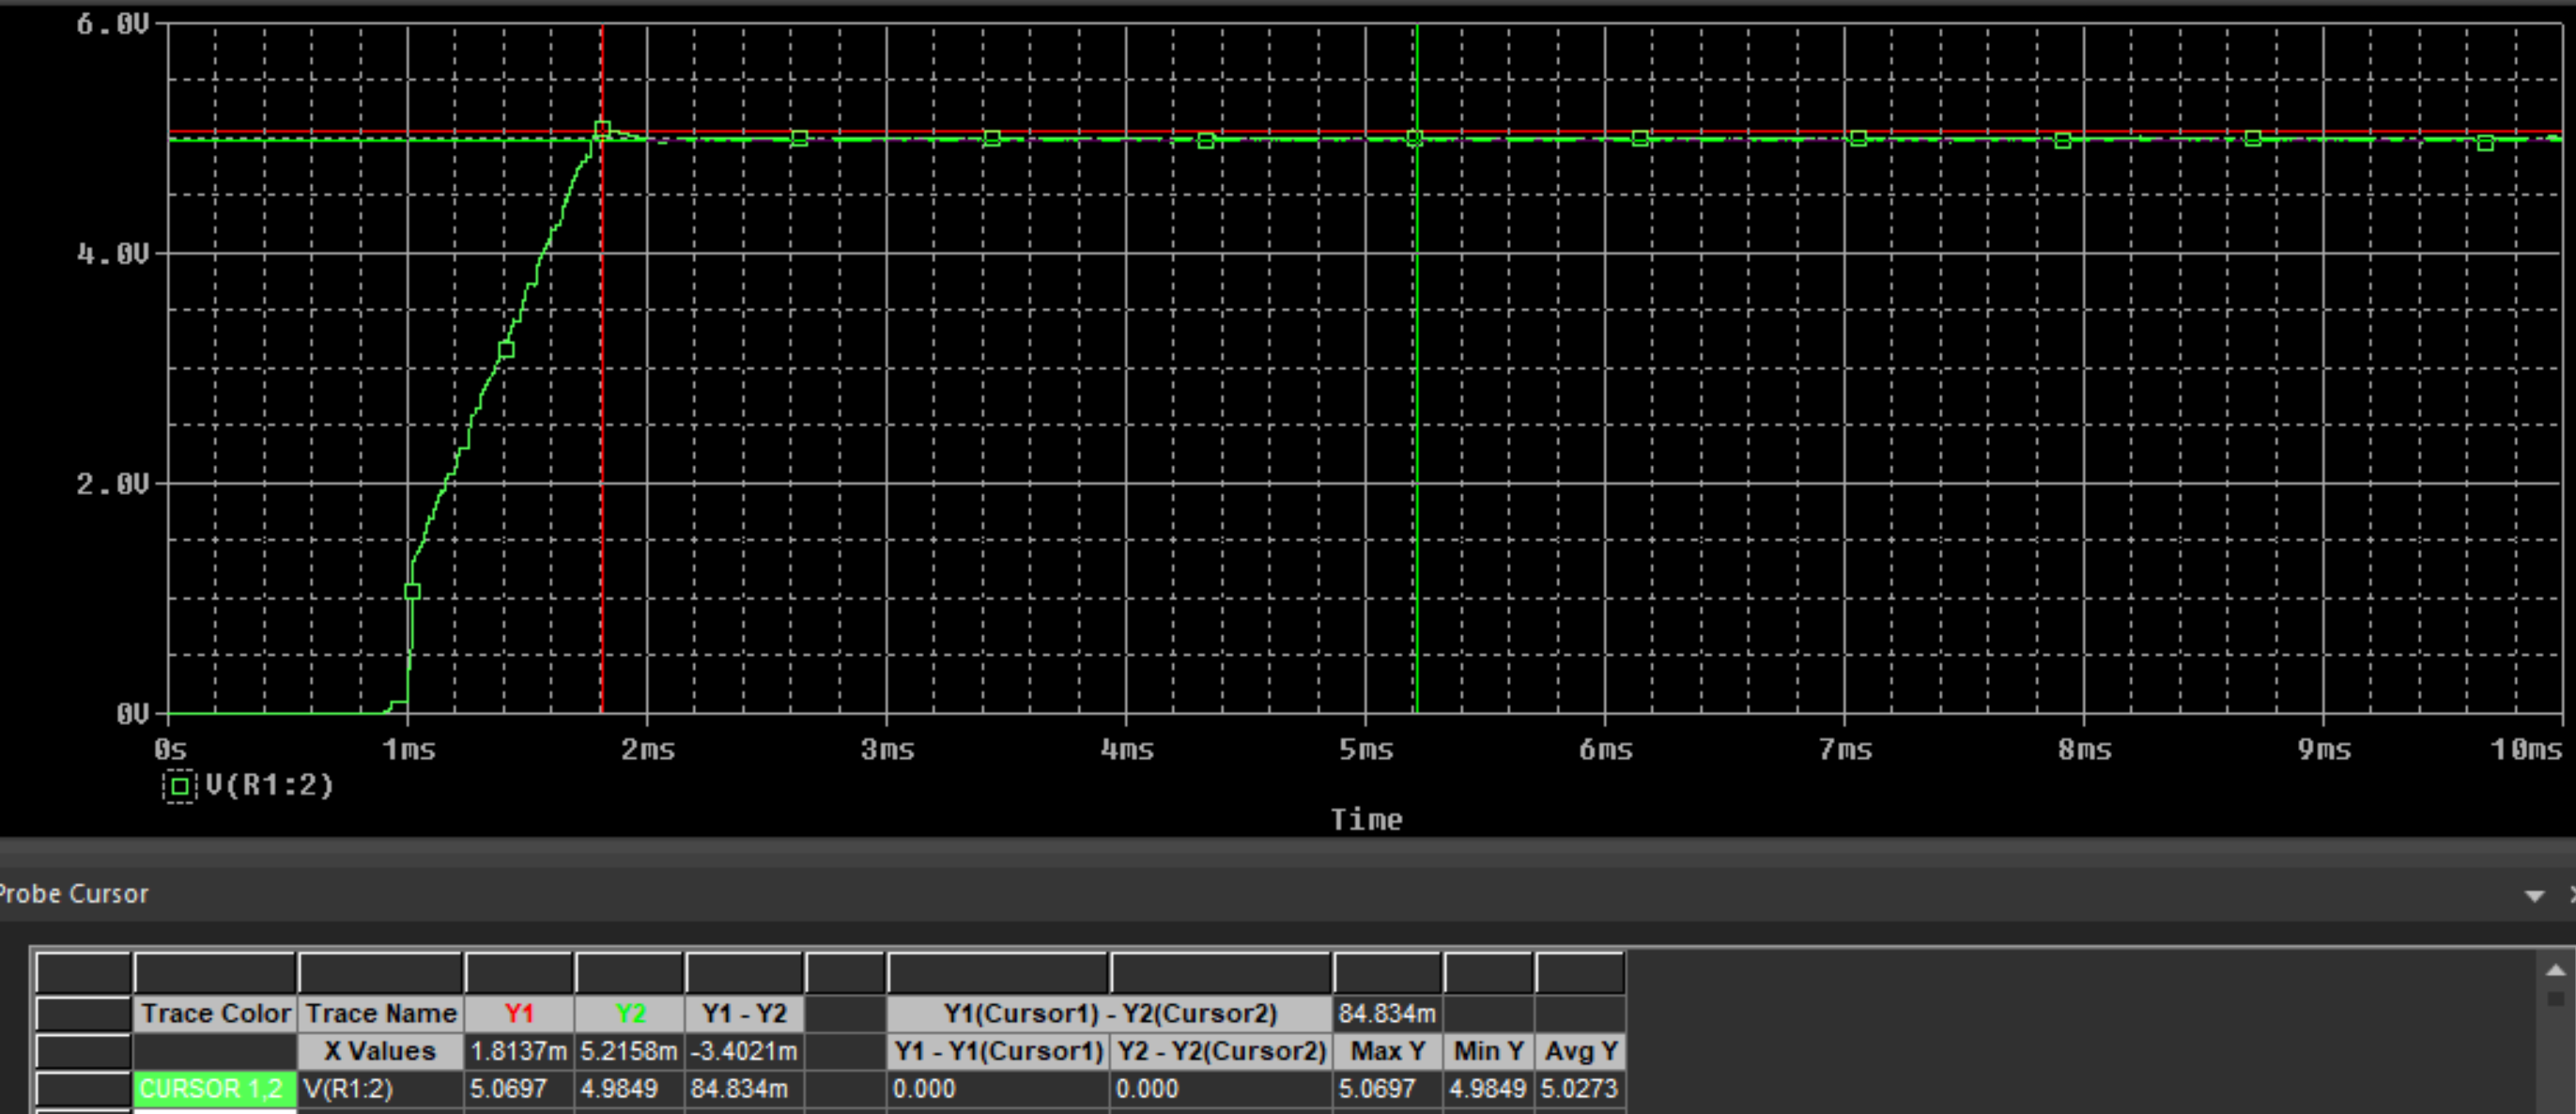
\includegraphics[scale=0.22]{graphics/ex10/f7.png}
    \caption{Kết quả mô phỏng của mạch trên}
\end{figure}

\textbf{Nhận xét và giải thích:} Đồ thị điện áp qua điện trở gần như không thay đổi trong 1ms đầu tiên, rồi tăng nhanh trong 1ms kế rồi ổn định ở mức điện áp 5 (V) nhưng còn chút gợn nhẹ với độ lệch khoảng 0,01 (V). Việc thêm cuộn cảm đã giúp cho mạch tăng điện áp nhanh hơn trong 2ms đầu và giúp cho điện áp ổn định hơn.
\pagebreak

Tiếp tục, thêm một diode Zener 5V vào mạch như hình 10.6, thay đổi tụ điện thành 220µF, thêm điểm đánh dấu dòng điện vào diode Zener, chạy lại mô phỏng và giải thích
vai trò của diode Zener trong mạch.

\begin{figure}[ht]
    \centering
    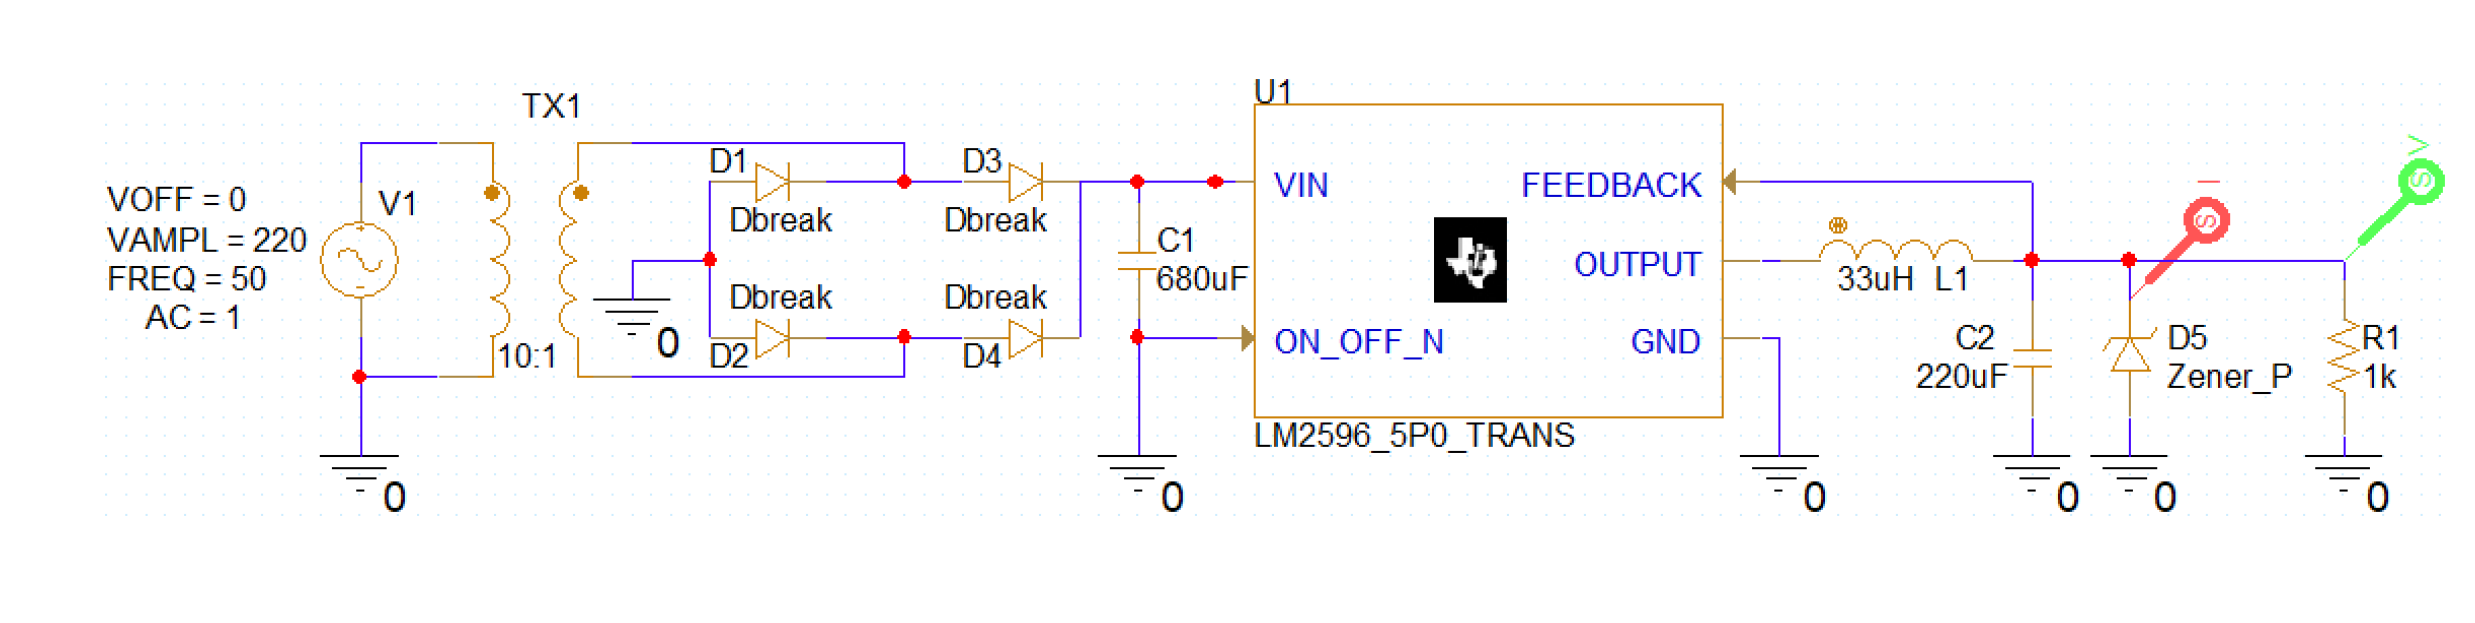
\includegraphics[scale=0.24]{graphics/ex10/f5.png}
    \caption{Một diode Zener 5V được thêm vào mạch}
\end{figure}

\textbf{Kết quả mô phỏng: }

\begin{figure}[ht]
    \centering
    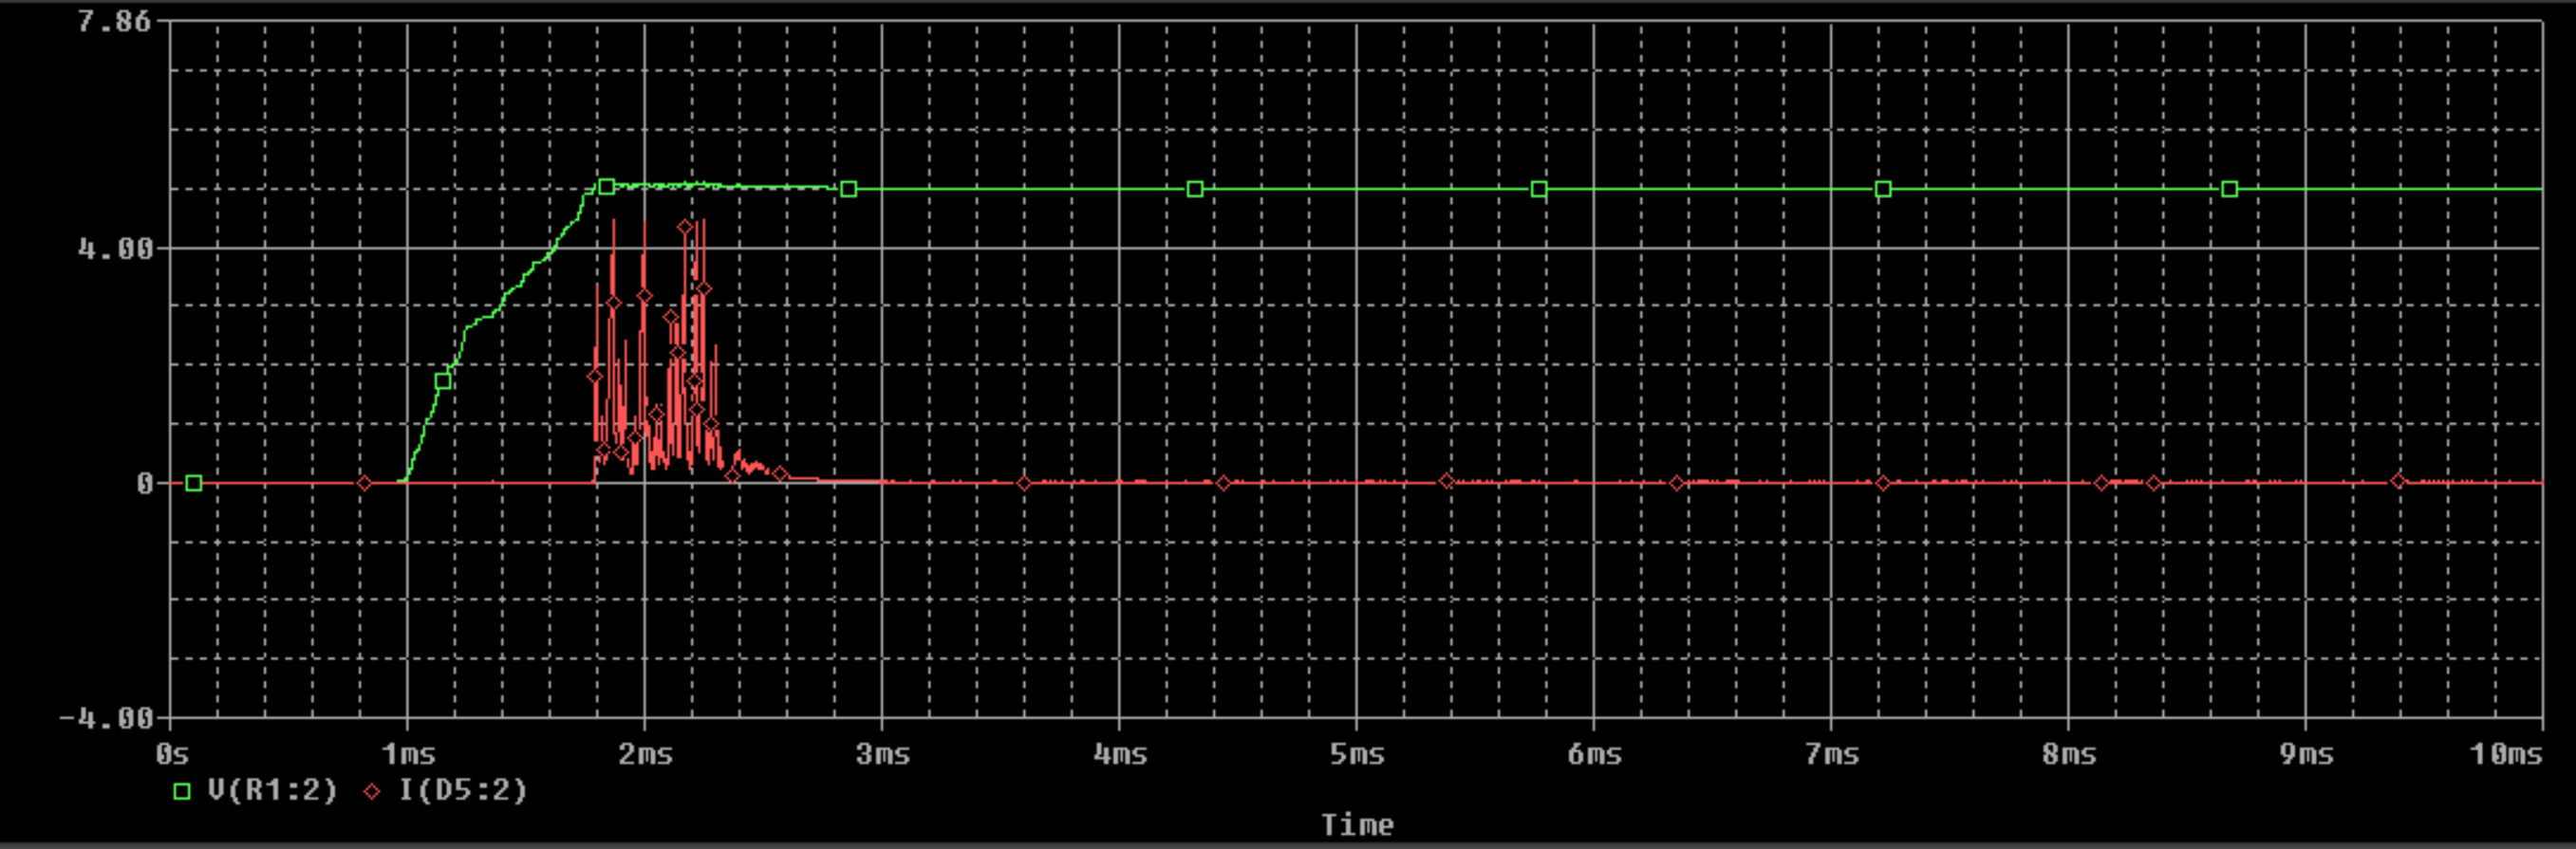
\includegraphics[scale=0.22]{graphics/ex10/f8.png}
    \caption{Kết quả mô phỏng của mạch trên}
\end{figure}

\textbf{Nhận xét và giải thích:} Đồ thị điện áp qua điện trở đã trở nên trơn hơn và ổn định hơn trước. Điều này là do việc thêm diode zener. Khi điện áp tại điện trở vượt qua 5(V), diode zener bắt đầu hoạt động và chống nhiễu, giúp điện áp luôn ổn định ở mức dưới 5 (V) (các gợn sóng màu đỏ trong hình biểu thị dòng điện tại diode zener khi điện áp tại điện trở vượt quá 5(V) ).




